% -----------------------------------------------------------------------------
% Description: Quantitative Results (Table 6, 7, 8 from paper)
% -----------------------------------------------------------------------------

% -----------------------------------------------------------------------------
% File: sections/04_results/1_performance.tex
% Description: Quantitative Results (Safe Colors: Blue/Red/Gray)
% -----------------------------------------------------------------------------

\begin{frame}{Quantitative Performance Analysis}
    \centering
    \vspace{-0.2cm}

    % --- Insight Box ---
    \begin{beamercolorbox}[sep=5pt, center, rounded=true, shadow=false, bg=blue!5]{insight}
        \small \textbf{Key Insight:} Dual-Model Fusion achieves the best balance, significantly boosting \textbf{Sensitivity} (+12.5\%) compared to the baseline.
    \end{beamercolorbox}

    \vspace{0.4cm}

    % --- Comparison Table ---
    \renewcommand{\arraystretch}{1.4}
    \setlength{\tabcolsep}{8pt}
    \resizebox{0.95\textwidth}{!}{%
    \begin{tabular}{lcccc}
        \toprule
        \textbf{Model Strategy} & \textbf{Accuracy} & \textbf{Precision} & \textbf{Sensitivity} & \textbf{F1-Score} \\
        \midrule

        % Base VGG16 (Grayed out)
        \textcolor{gray}{Base VGG16 ($L_1$)} & \textcolor{gray}{83.54\%} & \textcolor{gray}{90.91\%} & \textcolor{gray}{75.00\%} & \textcolor{gray}{82.19\%} \\

        % Tuned VGG16 (Normal)
        Tuned VGG16 ($L_2$) & 87.34\% & \textbf{94.12\%} & 80.00\% & 86.49\% \\

        \midrule

        % Fused Model (Highlighted with Standard Blue!10)
        % Using \cellcolor is safer than \rowcolor for specific templates
        \cellcolor{blue!10}\textbf{Fused VGG16 ($L_1 \lor L_2$)} &
        \cellcolor{blue!10}\textbf{89.87\%} &
        \cellcolor{blue!10}92.11\% &
        \cellcolor{blue!10}\textbf{\textcolor{red}{87.50\%}} &
        \cellcolor{blue!10}\textbf{89.74\%} \\
        \bottomrule
    \end{tabular}
    }

    \vspace{0.5cm}

    % --- Visual Metric Improvement (Mini Bar Chart) ---
    \begin{columns}
        \begin{column}{0.3\textwidth} \raggedleft \footnotesize \textbf{Sensitivity Gain:} \end{column}
        \begin{column}{0.6\textwidth}
            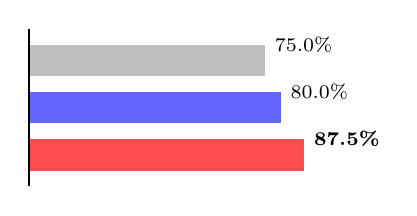
\begin{tikzpicture}
                % Base (Gray)
                \fill[gray!50] (0,0) rectangle (3.0, 0.4) node[right, black, font=\scriptsize] {75.0\%};

                % Tuned (Standard Blue - Safe)
                \fill[blue!60] (0,-0.6) rectangle (3.2, -0.2) node[right, black, font=\scriptsize] {80.0\%};

                % Fused (Red - The Winner)
                \fill[red!70] (0,-1.2) rectangle (3.5, -0.8) node[right, black, font=\bfseries\scriptsize] {87.5\%};

                % Y-Axis Line
                \draw[thick] (0,-1.4) -- (0,0.6);
            \end{tikzpicture}
        \end{column}
    \end{columns}
\end{frame}



% -----------------------------------------------------------------------------
% -----------------------------------------------------------------------------

\begin{frame}{Clinical Impact: Reducing Missed Diagnoses}
    \centering
    % 1. Tạo khoảng thở với tiêu đề slide (tránh bị dính)
    \vspace{0.3cm}

    % 2. Dùng [T] (Top align) để tiêu đề 2 bên luôn thẳng hàng
    \begin{columns}[T]

        % --- LEFT COLUMN: BASE MODEL ---
        \begin{column}{0.45\textwidth}
            \centering
            % Header Block
            \textbf{Base VGG16}
            \par\vspace{0.1cm}
            \hrule height 1pt % Đường kẻ phân cách ngang
            \vspace{0.3cm}

            \resizebox{0.9\textwidth}{!}{%
            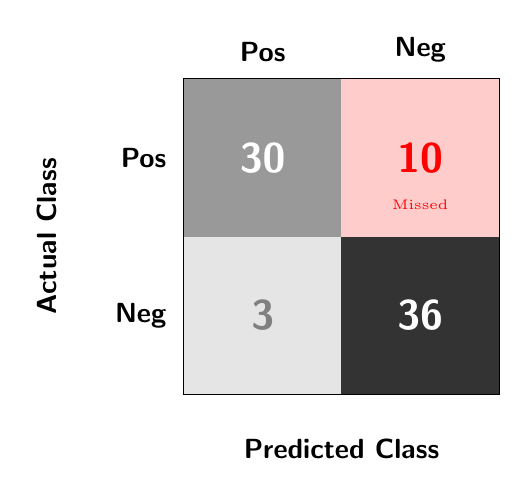
\begin{tikzpicture}[font=\sffamily\bfseries]
                % Grid
                \draw[thick] (0,0) rectangle (4,4);
                \draw[thick] (2,0) -- (2,4);
                \draw[thick] (0,2) -- (4,2);

                % --- LABELS (Fixed & Safe) ---
                % Axis Title: Dời hẳn sang x=-1.5 để ko dính Pos/Neg
                % anchor=south để căn chỉnh tâm chuẩn hơn khi xoay
                \node[rotate=90, anchor=south] at (-1.5, 2) {Actual Class};

                % Row Labels (Left side)
                \node[anchor=east] at (-0.1, 3) {Pos};
                \node[anchor=east] at (-0.1, 1) {Neg};

                % Column Labels (Top side)
                \node[anchor=south] at (1, 4.1) {Pos};
                \node[anchor=south] at (3, 4.1) {Neg};

                % X-Axis Label
                \node at (2, -0.7) {Predicted Class};

                % --- DATA ---
                % TP
                \fill[gray!80] (0,2) rectangle (2,4);
                \node[white, scale=1.5] at (1,3) {30};

                % FN (Missed)
                \fill[red!20] (2,2) rectangle (4,4);
                \node[red, scale=1.5] at (3,3) {10};
                \node[red, font=\tiny, align=center] at (3,2.4) {Missed};

                % FP
                \fill[gray!20] (0,0) rectangle (2,2);
                \node[gray, scale=1.5] at (1,1) {3};

                % TN
                \fill[black!80] (2,0) rectangle (4,2);
                \node[white, scale=1.5] at (3,1) {36};
            \end{tikzpicture}
            }
        \end{column}

        % --- MIDDLE: SEPARATOR ARROW ---
        \begin{column}{0.08\textwidth}
            \centering
            \vspace{2.5cm} % Đẩy mũi tên xuống giữa hình
            \Huge $\Rightarrow$
        \end{column}

        % --- RIGHT COLUMN: FUSED MODEL ---
        \begin{column}{0.45\textwidth}
            \centering
            % Header Block (Color Highlight)
            \textbf{\textcolor{blue}{Fused VGG16}}
            \par\vspace{0.1cm}
            {\color{blue} \hrule height 1pt} % Đường kẻ màu xanh
            \vspace{0.3cm}

            \resizebox{0.9\textwidth}{!}{%
            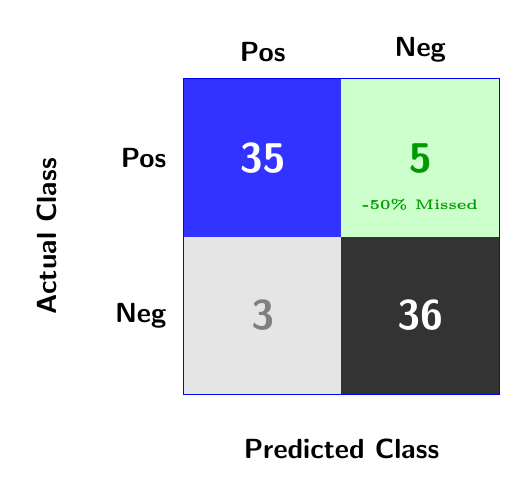
\begin{tikzpicture}[font=\sffamily\bfseries]
                % Grid (Blue Theme)
                \draw[thick, blue] (0,0) rectangle (4,4);
                \draw[thick, blue] (2,0) -- (2,4);
                \draw[thick, blue] (0,2) -- (4,2);

                % --- LABELS (Aligned with Left) ---
                \node[rotate=90, anchor=south] at (-1.5, 2) {Actual Class};
                \node[anchor=east] at (-0.1, 3) {Pos};
                \node[anchor=east] at (-0.1, 1) {Neg};
                \node[anchor=south] at (1, 4.1) {Pos};
                \node[anchor=south] at (3, 4.1) {Neg};
                \node at (2, -0.7) {Predicted Class};

                % --- DATA ---
                % TP
                \fill[blue!80] (0,2) rectangle (2,4);
                \node[white, scale=1.5] at (1,3) {35};

                % FN (Improved)
                \fill[green!20] (2,2) rectangle (4,4);
                \node[green!60!black, scale=1.5] at (3,3) {5};
                \node[green!60!black, font=\tiny, align=center] at (3,2.4) {\textbf{-50\% Missed}};

                % FP
                \fill[gray!20] (0,0) rectangle (2,2);
                \node[gray, scale=1.5] at (1,1) {3};

                % TN
                \fill[black!80] (2,0) rectangle (4,2);
                \node[white, scale=1.5] at (3,1) {36};
            \end{tikzpicture}
            }
        \end{column}
    \end{columns}

    \vspace{0.3cm}

    % Conclusion Box
    \begin{beamercolorbox}[sep=4pt, center, rounded=true, bg=green!10]{conclusion}
        \small \textbf{Impact:} Fusion strategy recovered \textbf{5 patients} (TP: $30 \to 35$) previously missed by the base model.
    \end{beamercolorbox}
\end{frame}